%% This is an example first chapter.  You should put chapter/appendix that you
%% write into a separate file, and add a line \include{yourfilename} to
%% main.tex, where `yourfilename.tex' is the name of the chapter/appendix file.
%% You can process specific files by typing their names in at the 
%% \files=
%% prompt when you run the file main.tex through LaTeX.

\chapter{Introduction}
Mercury (Hg) is a severe health hazard in the environment and in people, especially for fetuses and young children\cite{gibb_mercury_2014}. Moreover, mercury can travel great distances when released into the atmosphere, contaminating ecosystems, fish, birds, mammals, and human food chains \cite{esdaile_mercury_2018}.Recent estimates as seen of Figure\ref{fig:gma2018_hg-emissions_by-industry} indicate that about 37.7\% of global Hg emissions come from ASGM making it the most significant source of Hg pollution to the atmosphere and hydrosphere around the world\cite{unep_minamata_2019}. However, the amount of Hg released by ASGM activities and the extent to which it is transported regionally and globally is highly uncertain. While most of the Hg pollution from ASGM is local, its ability to travel across borders and contaminate distant ecosystems bolsters the case for concerted global efforts to combat Hg pollution in all forms, including ASGM. The Minamata Convention (MC) is one of the global efforts to combat Hg pollution in the world and its text is comprised of articles that also target ASGM Hg emissions. As evidenced by the MC's article 22 on the effectiveness evaluation of the MC, it is essential to have consistent and scientifically rigorous reporting about Hg releases and emissions from all emission sectors including the ASGM sector to create sound policies and management actions that will foster sustainable change. Furthermore, Cash et al. (2003) argue that science can influence social responses to public issues when relevant stakeholders view it as credible, salient, and legitimate. This thesis demonstrates how atmospheric modelling would add value to the effectiveness evaluation of the MC on ASGM Hg emission reductions and advocates for the expansion of global atmospheric monitoring networks particularly in the regions with high ASGM emissions. 

\begin{figure}[H]
  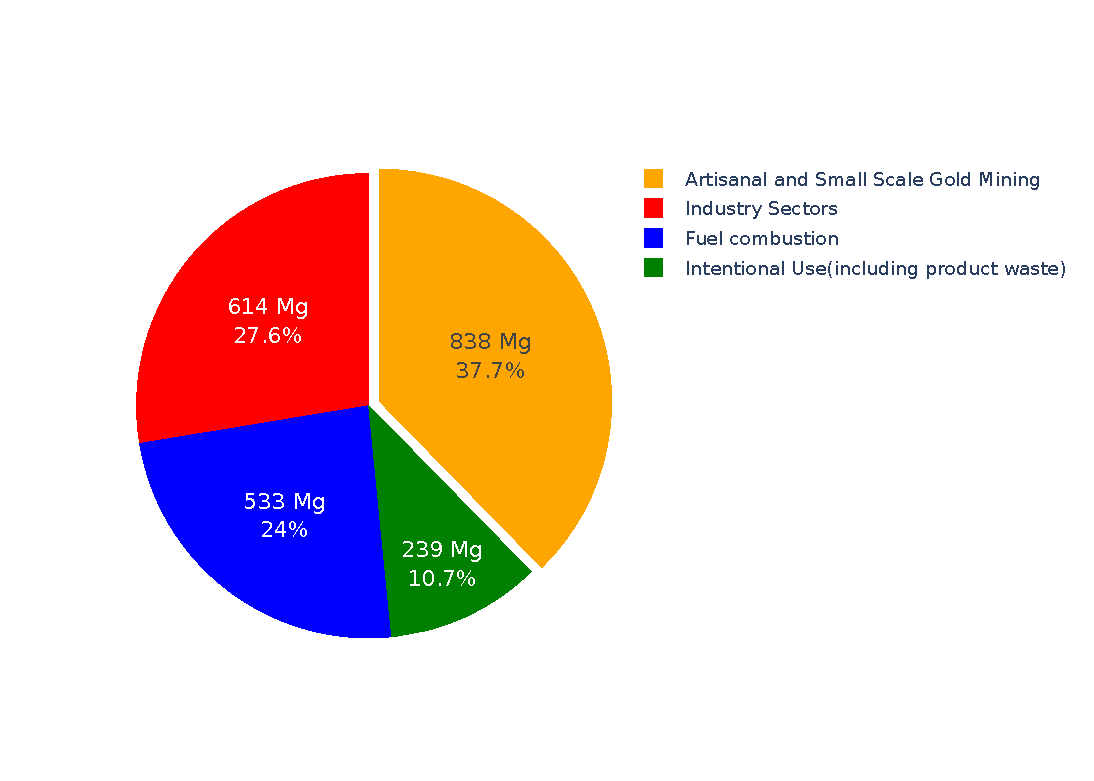
\includegraphics[width=\textwidth]{templates/figures/07-24-22_gma2018_hg-emissions_by-industry.pdf}
  \centering
  \caption{Pie chart showing the GMA 2018 ASGM \hg emission estimates for different sectors. ASGM is the sector with the highest Hg emissions (shown in orange) at 838 Mg followed by industry sectors (shown in red) at 614 Mg then fuel combustion (shown in blue) at 533 Mg, and finally intentional use sectors excluding ASGM (show in green) at 239 Mg \cite{united_nations_environment_programme_technical_2019}.}
  \label{fig:gma2018_hg-emissions_by-industry}
\end{figure}
\FloatBarrier

\section{Motivation}
\begin{flushleft}
More than 100 million people depend on artisanal and small-scale gold mining (ASGM) for their livelihood globally, particularly in the over 81 countries, predominantly in the global south where where ASGM exists.Additionally, ASGM is an essential source of income and an opportunity for rural development in the countries it exists where options and alternatives to ASGM for generating income to buy necessities of daily life are in short supply or none existent \cite{planetgold_planetgold_2021}. Furthermore, around 10 to 20 million (ASGM) miners are employed in the ASGM worldwide - about a third of them are women - and they provide 90\% of the global gold mining workforce and extract about 20\% of the world’s gold annually \cite{planetgold_planetgold_2021}. For example, in Peru, ASGM sustains the livelihoods of an estimated 1 million people, and between 300,000 and 500,000 miners were involved in Peru’s ASGM sector as of 2014. Despite being a vital source of livelihood for the communities that practice ASGM, its activities often lead to several environmental, human, and social harms. ASGM externalities include deforestation, tropical diseases such as malaria, dangerous and unsafe working conditions, crime and exploitation of indigenous communities, diesel and gasoline spills, and human trafficking in addition to the aforementioned Hg releases to the environment\cite{usaid_usaid_2020}. 
\end{flushleft}

\section{Artisanal and Small-Scale Gold Mining and Mercury Pollution}

\begin{flushleft} 
During ASGM, Hg is added to the gold ore to form a mercury-gold amalgam, a mixture of about equal amounts of Hg and gold\cite{united_nations_environment_programme_reducing_2012}. Heat is applied to the amalgam, which evaporates the Hg, leaving the gold behind. Gold extraction using this method is popular with the ASGM community since it is inexpensive, easy to use, and quick \cite{united_nations_environment_programme_reducing_2012}. Moreover, Hg is relatively effective at capturing gold when there are no other options, but often captures less than 40\% \cite{united_nations_environment_programme_developing_2015}. There is often a tremendous amount of Hg vapor in the air around amalgam burning sites, much higher than the World Health Organization(WHO) limit of 1.0 $\mu$g/m$^{3}$\cite{gibb_mercury_2014}. The emissions of Hg in ASGM are not only harmful to miners and members of their communities, but humans and ecosystems far away are also exposed to Hg risks because Hg travels globally through the atmosphere. As vaporized Hg settles in soil, rivers, bays, and oceans, anaerobic organisms transform it into methylmercury and water bodies can become contaminated with methylmercury. Methyl mercury is absorbed and ingested by phytoplankton, zooplankton, and fish and predator species such as sharks and swordfish that live a long time accumulate methylmercury and are usually the source of poisoning for people who eat fish. Figure \ref{fig:world_hg_emisions} shows how the anual average of the total Hg emissions from  all global anthropogenic Hg emissions sources. 
\end{flushleft}

\begin{figure}[H]
  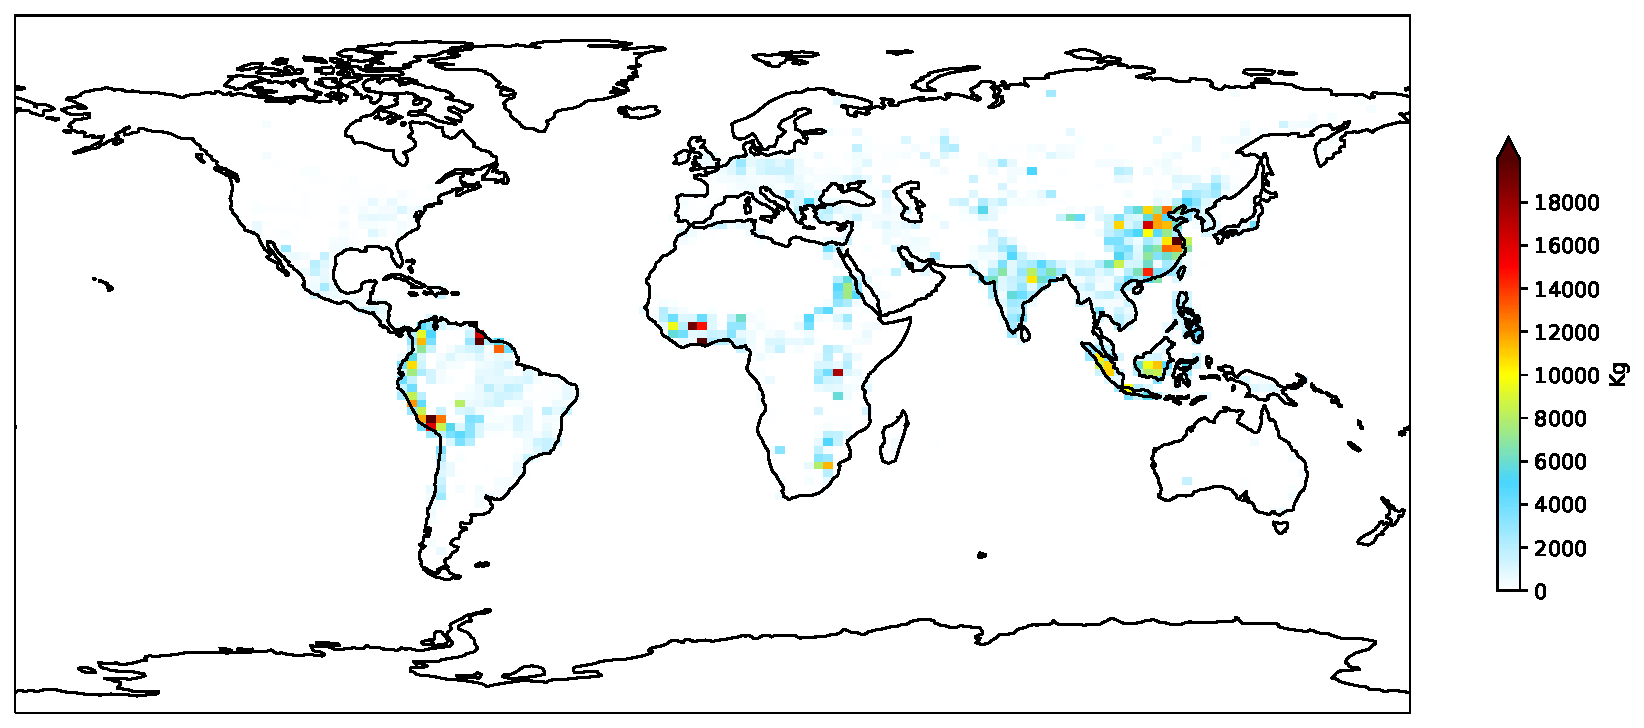
\includegraphics[width=0.8\textwidth]{templates/figures/06-12-22_total_Hg0-emissions-per-year_globally_001.pdf}
  \centering
  \caption{Spatial distribution of annual average Hg anthropogenic emissions for a year period between July 2014 and July 2015 \cite{united_nations_environment_programme_technical_2019}}
  \label{fig:world_hg_emisions}
\end{figure}
\FloatBarrier

\section{ASGM Measures in the Minamata Convention}
The MC is a global treaty was agreed upon at the fifth meeting of the Intergovernmental Negotiating Committee on Hg in Geneva, Switzerland in January 2013, and formally adopted in October that year in Kumamoto, Japan. Moreover, the treaty entered into force on 16 August 2017, 90 days after the 50\textsuperscript{th} instrument of ratification was deposited and currently has 137 parties to the convention\cite{unep_minamata_2019}. The goal of the MC is to to protect human health and the environment from the adverse effects of mercury and it affirmed that global action is essential to address the Hg pollution problem. Article 7 and Annex C of the MC target ASGM but, ASGM related issues such such as provisions on providing technical assistance and capacity building can be tackled through other articles in accordance with executing the main objective of the MC. Article 7 requires countries where Hg is used in ASGM to develop a National Action Plan (NAP) that details ways to reduce and, where possible, eliminate the use of Hg and Hg compounds. Each country should include in its NAP actions to stop some of the worst practices of ASGM, which include, among other things, (i) whole ore amalgamation, (ii) open burning of amalgam, (iii) burning of amalgam in residential areas (iv), and cyanide leaching in sediment or tailings to which Hg has been added without first removing the Hg \cite{unep_minamata_2019}. Moreover, countries are required to include in their NAPs baseline estimates of the quantities of Hg used in ASGM and the produced estimate should have an accuracy of $\pm$ 30\% and at worst $\pm$ 50\%\cite{programme_estimating_2017}. Rather than using generic strategies, countries must have a holistic approach to their NAPs, including policy, regulatory, institutional, technical, environmental, health, and socio-economic elements. Furthermore, international non-governmental organizations have developed programs such as the planetGold Project (led by UNEP and Conservation International with specific programs in 23 developing countries) to facilitate countries' implementation of Article 7 of the MC. A vital component of the MC is Article 22, which specifies a variety of information that must be included when conducting the effectiveness evaluation of the MC. The article states that "the Conference of the Parties shall, at its first meeting, initiate the establishment of arrangements for providing itself with comparable monitoring data on the presence and movement of Hg and Hg compounds in the environment as well as trends in levels of Hg and Hg compounds observed in biotic media and vulnerable populations." 

\section{Case Study Region}
\begin{flushleft}
Based on Yoshimura et al.'s (2021) estimate of mercury losses and gold production by ASGM, Latin America has the highest average ratio of mercury losses to gold production, 4.63, while Africa and Asia have the lowest at 1.96 and 1.23, respectively. Moreover, the GMA 2018 reported that ASGM Hg emissions in Latin America were the highest, and Figure \ref{fig:global_asgm_emissions_above_a_tone_barchart} shows that Peru is one of the top emitters of ASGM-related Hg and 60\% of the top 10 ASGM Hg emitting countries in the world are in Latin America  \cite{united_nations_environment_programme_technical_2019}. However, atmospheric Hg data from Latin America are rare; hence Hg dynamics in the region are not well understood. 
\end{flushleft}
\begin{figure}[H]
  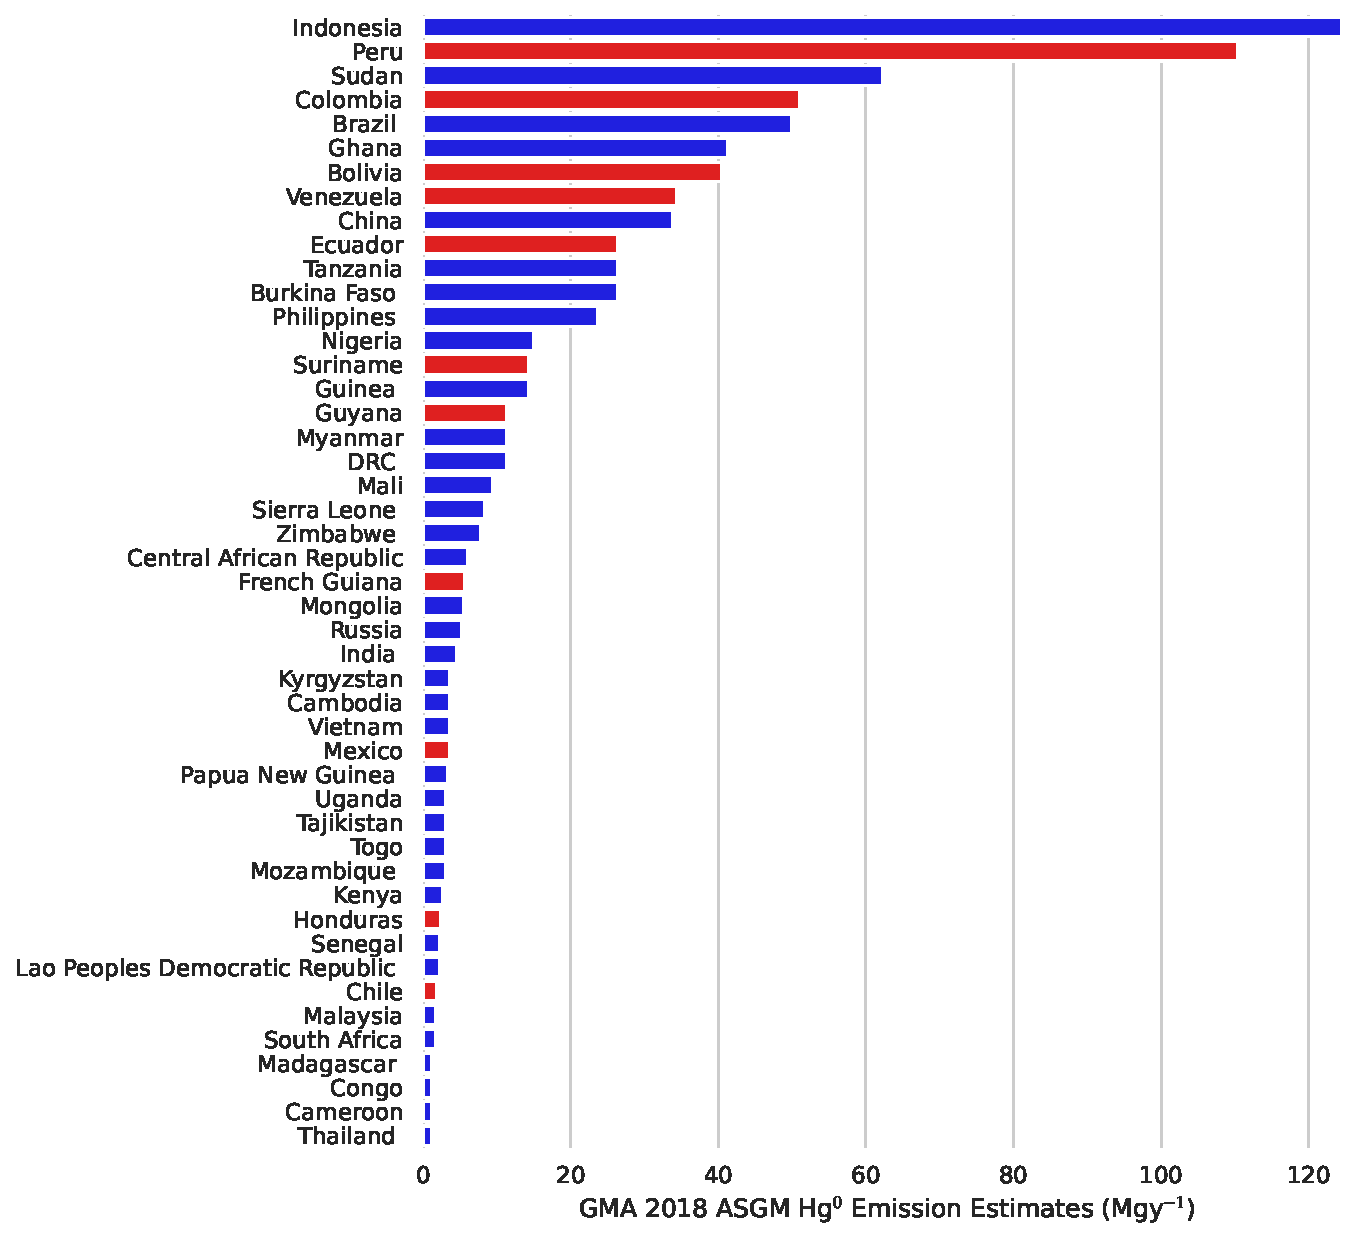
\includegraphics[width=\textwidth]{templates/figures/07-14-22_gma2018_top-asgm-emmiting-countries.pdf}
  \centering
  \caption{Bar chart showing the GMA 2018 ASGM \hg emission estimates for all countries in the world that have estimated ASGM \hg emissions above 1 Mg. The red bars highlight countries in Latin America \cite{united_nations_environment_programme_technical_2019}}
  \label{fig:global_asgm_emissions_above_a_tone_barchart}
\end{figure}
\FloatBarrier
\begin{flushleft}
Additionally, the Madre de Dios region in Peru was estimated to have released the largest quantities of Hg to the environment and the atmosphere\cite{agc_reporte_2017}. Madre de Dios which is shown by the red outline in Figure \ref{fig:PeruCS} is a rain forest region that lies between Bolivia and Brazil and covers roughly 85,000 square kilometers. The region's name is derived from the name of a major river that runs through it, and smaller streams and rivers cross through it to provide transportation and fishing for indigenous communities. Furthermore, these waterways are the main sites of ASGM and, subsequently, Hg contamination \cite{ashe_elevated_2012,agc_reporte_2017}. 
\begin{figure}[H]
  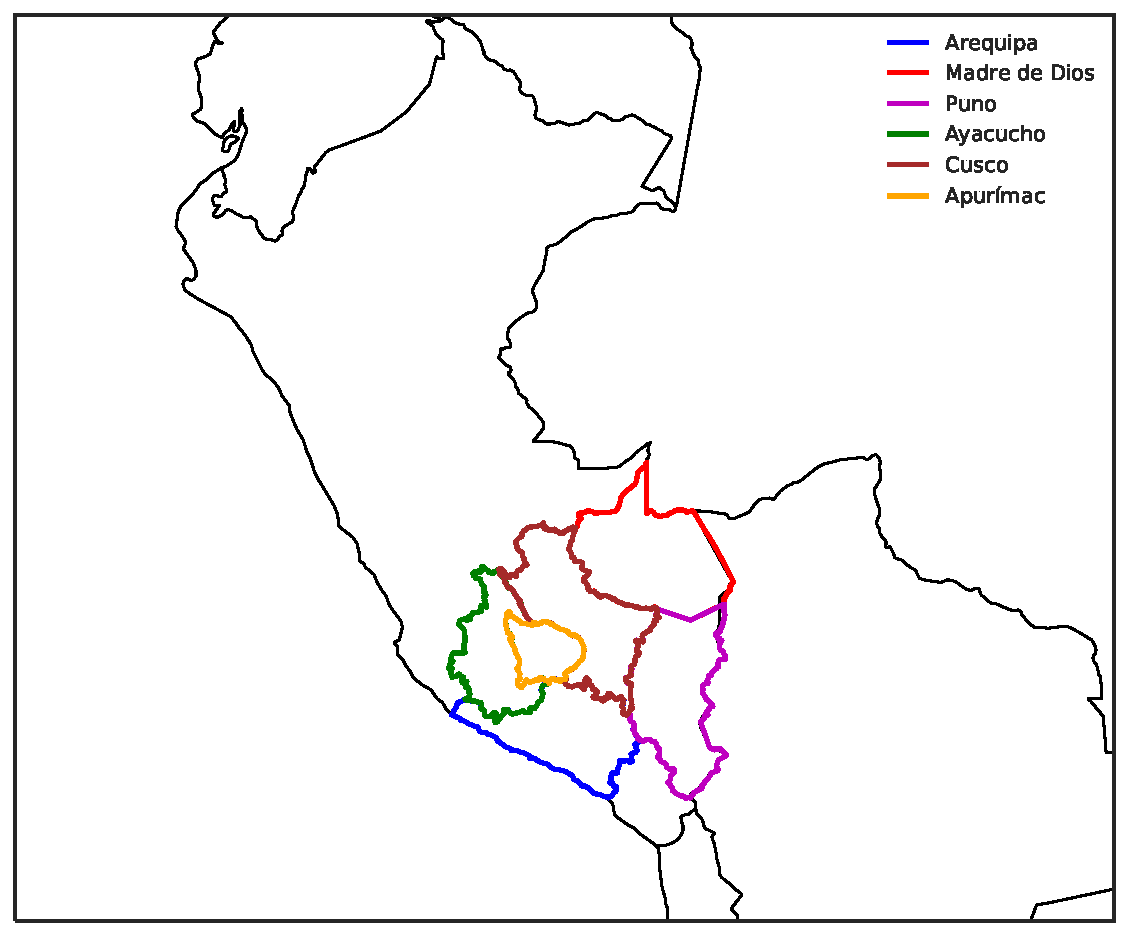
\includegraphics[width=0.6\textwidth]{templates/figures/Peru_Maps/CasestudyRegion.pdf}
  \centering
  \caption{Departments predicted to be the prominent sources of ASGM Hg releases according to the Artisanal Gold Council's  Inventory Report for the ASGM sector in Peru (2017) }
  \label{fig:PeruCS}
\end{figure}
\FloatBarrier

Hg has been extensively studied in Madre de Dios, both in people and in the environment and this thesis project complements previous studies and distinguishes itself from previous studies in this highly-studied region. It does this by investigating the extent to which the GEOS-Chem model can leverage existing measurements of Hg in the atmosphere and Hg emission estimates in published Hg global and national inventories to develop constraints on the amount of ASGM Hg emissions from the case study region in Peru. To develop a comprehensive understanding of how Hg pollution impacts the environment, long-term monitoring of ambient Hg data on a global scale is vital to assessing its emission, transportation, atmospheric chemistry, and deposition processes. Brasseur et al., (2017) prescribe that having a large ensemble of observations is vital for model evaluation; hence the lack of studies that analyze Latin America, Africa and South East Asia may be attributed to the fact that the aforementioned regions historically did not have enough Hg monitoring capacity. Although, a notable number of new atmospheric Hg monitoring programs have been set up and monitoring data from Latin America published in the past few years, Latin America, Africa and South East Asia are significantly behind Europe, and North America regarding capturing the relevant observation ensembles to track the evolution of Hg in the atmosphere. Regardless of the dearth of a large ensemble  of observations in Latin America, I present analysis and evaluation of atmospheric Hg concentrations simulated by the GEOS-Chem model with measurements recorded at multiple sites in Latin America including total gaseous mercury (TGM) measurements from the Global Mercury Observation System (GMOS) and gaseous elemental mercury (GEM) concentration data from a network of passive air samplers (PAS) distributed across Latin America. 

\end{flushleft}
\begin{flushleft}


\section{Thesis Questions}
According to Evers et al.(2016), country-specific actions under Article 7 of the MC will differ from country to country, and this variability poses a challenge to assessing the MC's effectiveness. Additionally, they argue that changes in the overall use of Hg in the global ASGM sector can be informed by progress in individual countries and suggest a compilation, visualization, and mapping of the respective data to track this progress across ASGM countries. Moreover, N.E Selin, (2014) highlighted that the existing global-scale monitoring networks for background Hg levels were at the time incapable of indicating whether the MC would lead to changes in the global biogeochemical cycling of Hg .She further argued that monitoring the effectiveness of policy requires better knowledge of and ability to explain baseline levels in the global biogeochemical cycle in the absence of policy, and track potential changes. This value added by baseline estimates of emissions to policy making is reflected in the MC's paragraph 3 of Article 7, which stipulates that each party that notifies the secretariat that (ASGM) and processing in its territory is more than insignificant shall develop and implement a national action plan (NAP) in accordance with annex C to the MC. In addition, annex C (d) states that the NAP shall include baseline estimates of the quantities of Hg used and the practices employed in ASGM and processing. As of this writing, 18 countries have submitted their respective NAPs and the estimates of how much Hg is used in their territories is shown on Figure\ref{fig:global-hg-emission-estimates_vs_nap_estimates}. However, the difference between the global estimates and the NAP estimates is very wide for some countries. 

\begin{figure}[H]
  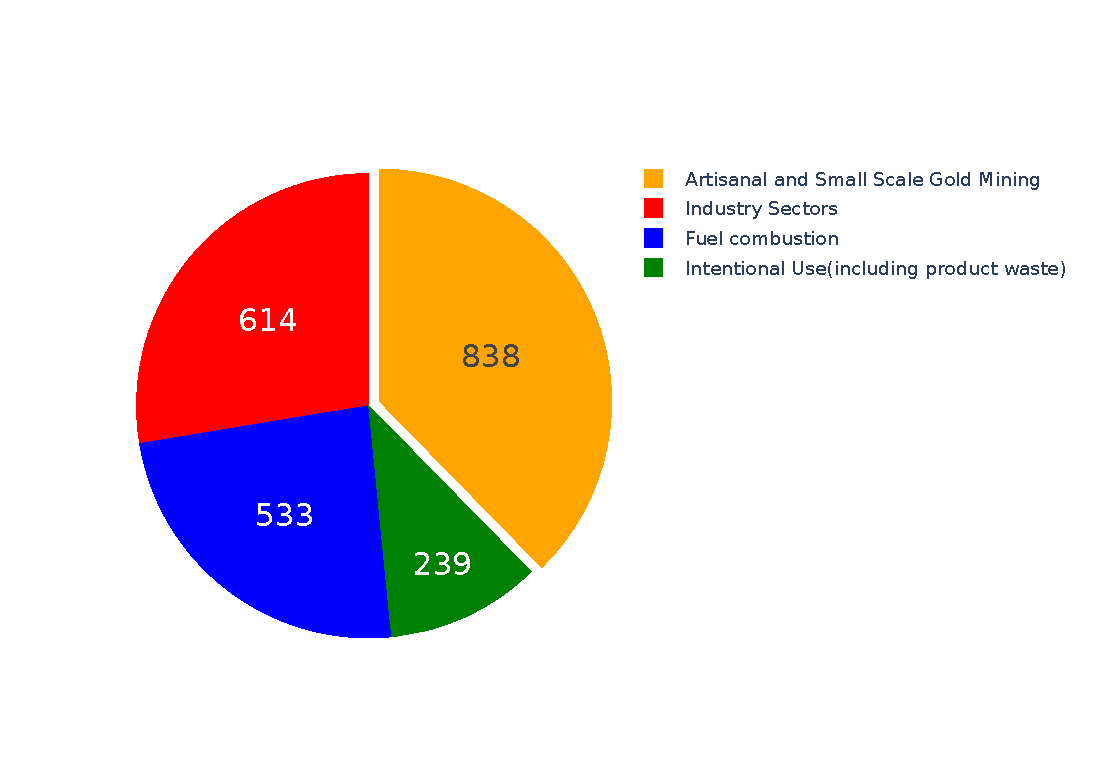
\includegraphics[width=\textwidth]{templates/figures/07-24-22_global-hg-emission-estimates_vs_nap_estimates.pdf}
  \centering
  \caption{Bar chart comparing the estimates of annual average Hg emissions predicted in the GMA 2018 inventory in light blue vs annual average Hg emissions baseline estimates (shown in dark blue) that were reported by the respective countries in their NAPs }
  \label{fig:global-hg-emission-estimates_vs_nap_estimates}
\end{figure}
\FloatBarrier
% Even though Peru has not yet submitted its national action plan, Figure [y] shows the differences between the global estimates of emissions and a local inventory that was produced by the Artisanal Gold Council in support of Peru's NAP.

 Therefore, in this thesis I seek to answer the following questions on the basis that simulating the amount of Hg in the atmosphere using chemical transport models (CTMs) such as GEOS-Chem can help integrate the data from individual countries with atmospheric measurement to provide an additional tool for tracking progress thus evaluating the effectiveness of the MC:
\begin{enumerate}
  \item To what extent can regional atmospheric modeling and monitoring help reconcile the differences in the current global estimates of emissions and national emissions?
  \item What kinds of regional monitoring networks are essential to improve the usefulness of models in evaluating the effectiveness of the MC?
  \item Which policies are essential to catalyze action towards the expansion of regional monitoring, particularly in the regions where ASGM emissions are the dominant source?
\end{enumerate}
\end{flushleft}
% CTMs provide an approximation of the behavior of various chemical species in the atmosphere which enables understanding of the real world and creates opportunities for future predictions. Models and observation networks have a symbiotic relationship that is one of the cornerstone ingredients of the multidisciplinary frameworks for producing scientific information and knowledge that is salient, credible and legitimate to inform the public and policy makers.



 
\section{Organization}
Addressing ASGM sub-sector issues requires ways to transform its negative impacts into enhanced positive ones, maximize ASGM's contribution to poverty reduction, and create resilient communities. This introductory chapter has provided a general background on ASGM in relation to Hg emissions. Chapter 2 discusses the value atmospheric added by atmospheric models to the Hg emission estimation task that must be carried out under the MC. The strengths and limitations of the GEOS-Chem model are highlighted, and strategies to improve the model's usefulness are presented. Chapter 3 presents one of the strategies for improving GEOS-Chem's usefulness in producing top-down estimates of ASGM Hg emissions. Furthermore, top-down estimates of ASGM Hg emissions from Some regions in Peru are produced. Chapter 4 presents policy recommendations and conclusions to address the third research question.



%\section{Organization}